\section{Results}
\label{sec:results}

\subsection{RQ1: recognition and selective risk}
The template matcher required a conservative operating point. Calibration selected $\tau=0.08$; on the 2,610 evaluation rows, it accepted 292 predictions and routed 2,318 to review. Coverage was 11.19\% (cluster-bootstrap 95\% interval 5.86\%--16.97\%), with no accepted error observed. The corresponding cluster-bootstrap interval for accepted accuracy was 100\%--100\%; this degenerate interval reflects the deterministic sample and does not establish a zero population error rate.

The HOG--linear-SVM changed the operating trade-off. Its calibration split already met the 1\% risk target at $\tau=0$, so the frozen selector accepted all 2,610 evaluation rows. It correctly classified 2,605, giving 99.81\% accepted accuracy and 0.19\% selective risk. Cluster resampling placed the risk interval at 0.038\%--0.346\% and the accepted-accuracy interval at 99.62\%--99.96\% (Table~\ref{tab:selective-models}). The result supports HOG--SVM as the evaluated digit recognizer; it does not support a claim of recognition novelty.

\begin{table}[t]
  \centering
  \caption{Calibration-selected operating points on the seed-disjoint evaluation split. Confidence intervals reported in the text resample 90 base units rather than 2,610 rows.}
  \label{tab:selective-models}
  \begingroup
  \footnotesize
  \setlength{\tabcolsep}{3pt}
  \begin{tabular}{lrrrr}
\toprule
Model & Cov. (\%) & Acc. (\%) & Risk (\%) & Review (\%) \\
\midrule
Template matcher & 11.2 & 100.00 & 0.00 & 88.8 \\
HOG--SVM & 100.0 & 99.81 & 0.19 & 0.0 \\
\bottomrule
\end{tabular}

  \endgroup
\end{table}

\begin{figure}[t]
  \centering
  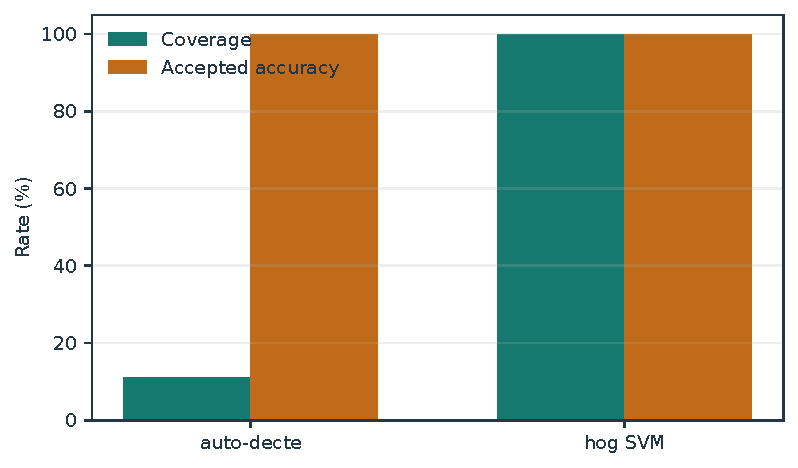
\includegraphics[width=0.76\textwidth]{figures/generated/model_selective_comparison.pdf}
  \caption{Coverage and conditional accepted accuracy for the two calibration-selected recognizer--gate combinations.}
  \label{fig:selective-models}
\end{figure}

The template gate remains informative as a stress case. Figure~\ref{fig:coverage-risk} shows that its full-coverage end incurred roughly 25\% selective risk; the first threshold with zero observed accepted error was $\tau=0.07$, at 14.83\% coverage. Severe perspective distortion and occlusion reduced its coverage to 3.33\%. Thus, selection prevented many weak template predictions from auto-passing, but the stronger HOG representation removed most of that synthetic-regime trade-off.

\begin{figure}[t]
  \centering
  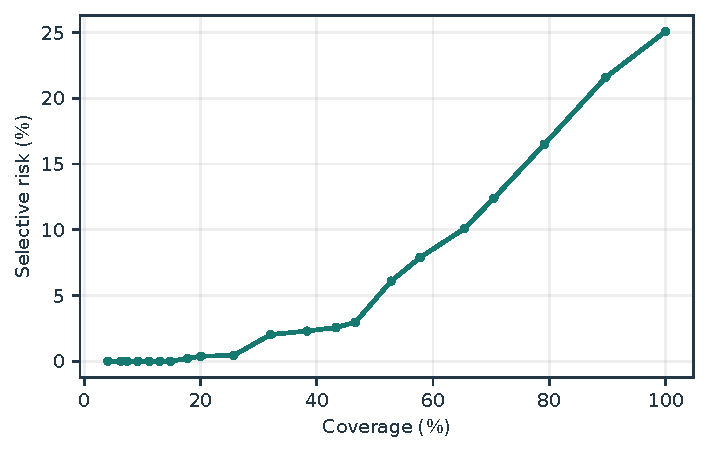
\includegraphics[width=0.76\textwidth]{figures/generated/coverage_risk.pdf}
  \caption{Template-matcher coverage--risk curve. The dashed operating point was selected on calibration data before evaluation.}
  \label{fig:coverage-risk}
\end{figure}

\subsection{RQ2: whole-form integration}
Across the 300 evaluation form--condition rows, template identification succeeded on 80\% and ArUco alignment succeeded on 80\%; both succeeded together on 180 rows (60\%). Across all conditions, digit accuracy was 86.03\%, OMR accuracy was 100\%, and complete-form success was 60\% (Table~\ref{tab:whole-form}). All 60 clean, 60 perspective, and 60 JPEG rows were completely correct. Gaussian blur preserved alignment and 100\% field accuracy but prevented QR identification on all 60 rows. Rotation preserved QR identification but prevented marker alignment on all 60 rows and reduced digit accuracy to 30.17\%. These complementary failures explain why the two marginal component rates exceed their joint rate and why the complete endpoint is 60\%.

\begin{table}[t]
  \centering
  \caption{Whole-form evaluation over 300 form--condition rows per variant. Complete success requires template identity, alignment, and all 20 fields correct.}
  \label{tab:whole-form}
  \begingroup
  \footnotesize
  \setlength{\tabcolsep}{3pt}
  \begin{tabular}{lrrrrr}
\toprule
Variant & QR (\%) & Align (\%) & Digit (\%) & OMR (\%) & Complete (\%) \\
\midrule
full\_pipeline & 80.0 & 80.0 & 86.0 & 100.0 & 60.0 \\
without\_qr & 0.0 & 80.0 & 86.0 & 100.0 & 0.0 \\
without\_aruco & 80.0 & 0.0 & 69.4 & 99.0 & 0.0 \\
\bottomrule
\end{tabular}

  \endgroup
\end{table}

Suppressing QR identification left field recognition unchanged but made the complete endpoint unattainable. Suppressing ArUco alignment reduced digit accuracy from 86.03\% to 69.43\% and OMR accuracy from 100\% to 99.03\%; complete-form success again fell to zero. Figure~\ref{fig:whole-form} separates the component rates so the endpoint's conjunctive definition is explicit.

\begin{figure}[t]
  \centering
  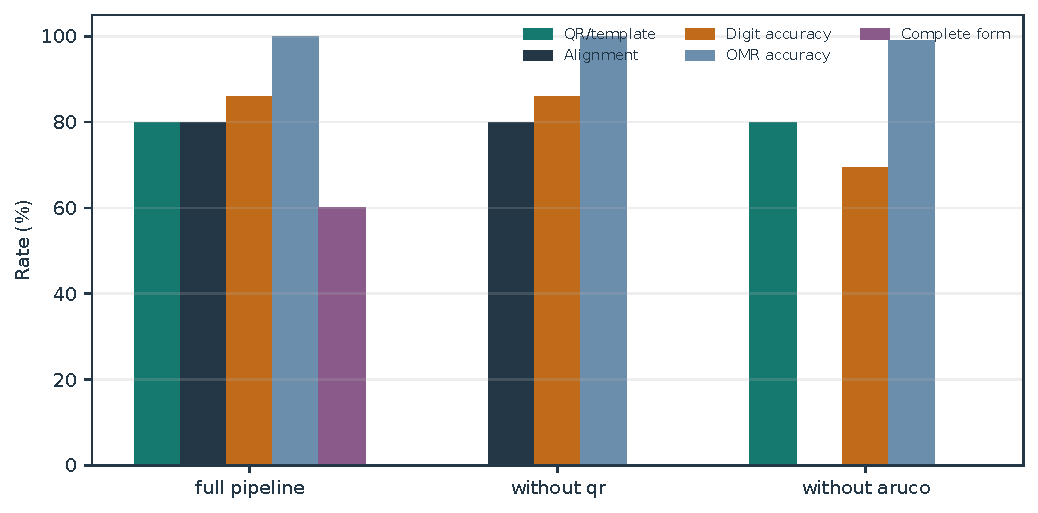
\includegraphics[width=0.82\textwidth]{figures/generated/whole_form_ablation.pdf}
  \caption{Whole-form component ablations. Removing a component required by the endpoint forces complete success to zero; field metrics show the additional recognition effect of missing alignment.}
  \label{fig:whole-form}
\end{figure}

\subsection{RQ3: authority-boundary faults}
All six controlled cases left the pre-existing fact unchanged and produced complete audit evidence. Wrong recognition and language-model outputs remained candidates, irrelevant retrieval remained a reference, stale review and duplicate evidence raised their designated exceptions, and all 12 attempted direct fact-write paths were absent from the three machine-facing services.

The candidate-isolation ablation supplied an incorrect value of 999. Under normal wiring, recording the candidate did not change the fact. Under test-only unsafe wiring that granted the same value access to the review service, the fact changed. This contrast locates containment in capability separation rather than in the injected value or recognizer behavior.

Randomized stress testing repeated five fault families 100 times each. All 500 trials were contained (Table~\ref{tab:fault-stress}). This expands the evidence beyond one example per family, although it remains an application-path test rather than a penetration test, formal proof, or assessment of host compromise.

\begin{table}[t]
  \centering
  \caption{Seeded randomized trust-boundary stress test.}
  \label{tab:fault-stress}
  \begin{tabular}{lrr}
\toprule
Fault family & Contained & Trials \\
\midrule
wrong\_recognition & 100 & 100 \\
wrong\_llm\_suggestion & 100 & 100 \\
irrelevant\_retrieval & 100 & 100 \\
stale\_human\_replay & 100 & 100 \\
duplicate\_evidence & 100 & 100 \\
\bottomrule
\end{tabular}

\end{table}

\subsection{RQ4: executable workflow and reproducibility}
Each of the 60 clean evaluation forms traversed the complete application workflow. The runner imported the original image, stored 20 recognition candidates, programmatically submitted known synthetic labels through the review service, created fact version~1, exported an XLSX file, and queried the reverse trace. All 60 workflows succeeded, accounting for 1,200 persisted candidate attempts. This verifies the software path but not human-review effectiveness. AI-disabled operation, duplicate rejection, stale-version rejection, and reverse tracing also passed.

The final verification run passed 77 automated tests, Ruff checks, and mypy checks. The artifact manifest contains 27 hashed outputs, records source commit \texttt{195355a}, and reports a clean tracked source state at generation time. Service microbenchmarks and the full perturbation table are supplied in the supplementary material because they do not measure end-to-end reviewer latency.
